\documentclass[12pt,letterpaper]{article}
\usepackage{pdfpages}
\usepackage{fancyhdr}
\usepackage[colorlinks=true, urlcolor=blue, linkcolor=blue]{hyperref}
\usepackage{graphicx}
\usepackage[top=1.4in, left=0.5in, right=0.5in, bottom=0.8in]{geometry}
\usepackage[T1]{fontenc}
\usepackage{helvet}
\pagestyle{fancy}
\renewcommand{\headrulewidth}{0pt}
\renewcommand{\footrulewidth}{0pt}
\setlength{\parindent}{0em}
\setlength{\parskip}{1em}


\fancyfoot[C]{\setlength{\unitlength}{1in}\begin{picture}(5,0)\put(-1.8,-1){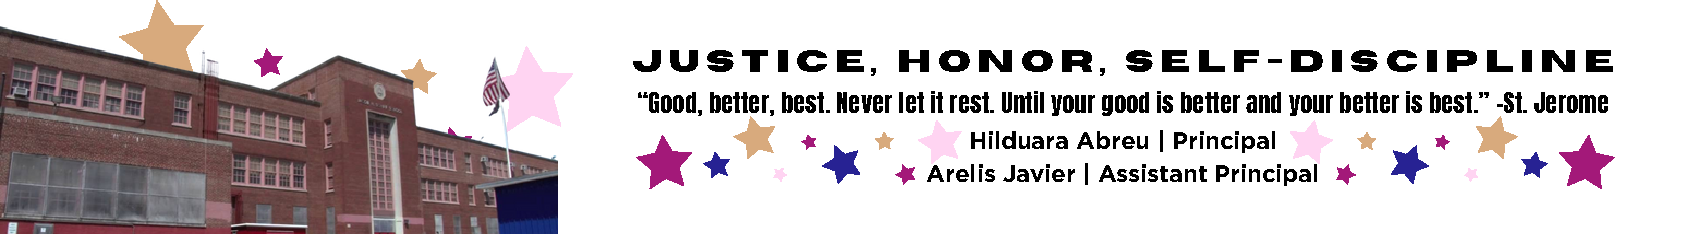
\includegraphics[width=8.8in,height=1.3in]{logo-1}}\end{picture}}
\fancyhead[C]{\setlength{\unitlength}{1in}\begin{picture}(5,0)\put(-1.9,-1){
\includegraphics[width=8.9in,height=1.3in]{logo-2}}\end{picture}}

\pagenumbering{gobble}
\addtolength{\evensidemargin}{-2in}
\addtolength{\topmargin}{-0.5in}
\addtolength{\textwidth}{0in}
%%%%%%%%%%%%%%%%%%%%%%%%%%%%%%%%%%%%%%%%%%%%%%%%%%%%%%%%%%%%%%%%%%

\begin{document}
\vspace*{0.5in}
School Website: \href{https://www.ps192.org}{www.ps192.org}

\textbf{Principal's Message February 2024}

Dear Parents or Guardians,

In accordance with our agenda for the month of February, we will be commemorating Valentine’s Day and observing the Mid-Winter Recess. The school will be closed from February 19th to February 23rd. We encourage you to consider various enriching activities for your children during this period, such as exploring the diverse museums our city offers or engaging with the events and resources at the Public Library, including borrowing books for home reading.
 
Please be informed that PS192 has a comprehensive schedule of events and activities planned around the recess. The following are key dates and events:
\begin{itemize}
\item Applications for 3K, Pre-K, Kindergarten, and Middle School for the 2024-2025 academic year are due.
\item Coffee with the Principal, Parent Association meeting, and Valentine’s Day Celebration will take place on February 14th in the Gymnasium at 8:00 a.m.
\item Graduation Meetings are scheduled for February 29th, with Pre-K \& Kindergarten from 2:30 p.m. to 3:00 p.m., and 5th Grade from 3:20 p.m. to 4:00 p.m. in the Library.
\end{itemize}

We cordially invite you to establish a weekly dialogue with your child’s teacher, utilizing email, our school website, or ClassDojo, to discuss and monitor your child’s social-emotional and academic growth. Your proactive involvement is greatly valued and plays a crucial role in their educational journey.

We extend our best wishes for a tranquil and enjoyable Mid-Winter Recess to all families.

Warm regards,


\includegraphics[width=0.2\textwidth]{hil_signature}

\textbf{Hilduara Abreu}

\textbf{Principal P.S. 192}

\textit{The School of Joyful Learning!}

\newpage
\vspace*{.5in}
Nuestro Sitio Web: \href{https://www.ps192.org}{www.ps192.org}

\textbf{Mensaje de La Directora Para Febrero 2024}

Estimados padres o tutores,

De acuerdo con nuestra agenda para el mes de febrero, estaremos conmemorando el Día de San Valentín y observando el Receso de Medio Invierno. La escuela estará cerrada del 19 al 23 de febrero. Le recomendamos que considere diversas actividades enriquecedoras para sus hijos durante este período, como explorar los diversos museos que ofrece nuestra ciudad o participar en los eventos y recursos de la Biblioteca Pública, incluido el préstamo de libros para leer en casa.
 
Tenga en cuenta que PS192 tiene un calendario completo de eventos y actividades planificadas durante el receso. Las siguientes son fechas y eventos clave:
\begin{itemize}
\item Las solicitudes para 3K, Pre-K, Kindergarten y Middle School para el año académico 2024-2025 están vencidas.
\item El café con el director, la reunión de la asociación de padres y la celebración del día de San Valentín se llevarán a cabo el 14 de febrero en el gimnasio a las 8:00 a. m.
\item El café con el director, la reunión de la asociación de padres y la celebración del día de San Valentín se llevarán a cabo el 14 de febrero en el gimnasio a las 8:00 a. m.
\item Las reuniones de graduación están programadas para el 29 de febrero, con Pre-K y Kindergarten de 2:30 p.m. a 3:00 p.m., y 5to Grado de 3:20 p.m. a 4:00 p.m. en la biblioteca.
\end{itemize}

Le invitamos cordialmente a establecer un diálogo semanal con el maestro de su hijo, utilizando el correo electrónico, el sitio web de nuestra escuela o ClassDojo, para discutir y monitorear el crecimiento socioemocional y académico de su hijo. Su participación proactiva es muy valorada y juega un papel crucial en su viaje educativo.
\newpage
\vspace*{.5in}
Extendemos nuestros mejores deseos para que todas las familias disfruten de un receso de mediados de invierno tranquilo y agradable.

Un cordial saludo,


\includegraphics[width=0.2\textwidth]{hil_signature}

\textbf{Hilduara Abreu}

\textbf{Principal P.S. 192}

\textit{The School of Joyful Learning!}
\end{document}
